\chapter{Specifikacija programske potpore}
		
	\section{Funkcionalni zahtjevi}
			
			\noindent \textbf{Dionici:}
			
			\begin{packed_enum}
				
				\item Neregistrirani korisnik
				\item Registrirani korisnik
				\begin{packed_enum}
					\item Vlasnik pasa
					\item Čuvar pasa
				\end{packed_enum}
				\item Administrator 				
				\item Razvojni tim
				
			\end{packed_enum}
			
			\noindent \textbf{Aktori i njihovi funkcionalni zahtjevi:}
			
			
			\begin{packed_enum}
				\item  \underbar{Neregistrirani korisnik (inicijator) može:}
				
				\begin{packed_enum}
					
					\item Pregledavati objavljene zahtjeve i oglase te njihove pojedinosti (lokacija, period čuvanja itd.)
					\item Registrirati se u sustav, stvoriti novi korisnički račun za koji mu trebaju ime, prezime, korisničko ime, e-mail adresa, lozinka i uloga.
				\end{packed_enum}
				
				\item  \underbar{Registrirani korisnik (inicijator) može:}
				
				\begin{packed_enum}
					
					\item Pregledavati osobne podatke
					\item Odjaviti se s korisničkog računa i prijaviti se nekim drugim računom
					\item Pregledavati pristigle ponude i povijest ponuda
					\item Pregledavati trenutna čuvanja i stupiti u kontakt s drugim korisnikom
					\item Imati ulogu vlasnika pasa:
					\begin{packed_enum}
						\item Spremiti podatke o svom psu
						\item Pregledavati svoje pse
						\item Pregledavati sve odobrene oglase čuvara pasa i sve odobrene zahtjeve drugih vlasnika pasa
						\item Pregledavati vlastite zahtjeve
						\item Stvarati novi zahtjev za čuvanje pasa
						\item Pronaći najbolji odabir čuvara pasa
						\item Ocjenjivati uslugu čuvara pasa
					\end{packed_enum}
					\item Imati ulogu čuvara pasa:
					\begin{packed_enum}
						\item Pregledavati sve odobrene zahtjeve vlasnika pasa i sve odobrene oglase drugih čuvara pasa
						\item Pregledavati vlastite oglase
						\item Stvarati novi oglas za čuvanje pasa
						\item Pronaći najbolji odabir vlasnika pasa
						\item Ocjenjivati ponašanje psa
						
					\end{packed_enum}
					\item Imati ulogu vlasnika i čuvara pasa:
					\begin{packed_enum}
						\item Ima sve navedene funkcionalnosti vlasnika pasa i čuvara pasa
					\end{packed_enum}
				\end{packed_enum}
			
				\item \underbar{Administrator (inicijator) može:}
				\begin{packed_enum}
					\item Obavljati sve funkcionalnosti registriranog korisnika
					\item Dodijeliti administratorsku ulogu drugim korisnicima
					\item Odobriti ili odbaciti zahtjev/oglas
					\item Blokirati korisnike koji narušavaju pravila sustava
				\end{packed_enum}
			
				\item \underbar{Baza podataka (sudionik) može:}
				\begin{packed_enum}
					\item Pohraniti sve podatke o registriranim korisnicima i njihovim ulogama
					\item Pohraniti sve podatke o psima
					\item Pohraniti sve podatke o stvorenim zahtjevima i oglasima
					\item Pohraniti podatke o mogućima aktivnostima sa psima
				\end{packed_enum}
			
			\end{packed_enum}
			
			\eject 
			
			
				
			\subsection{Obrasci uporabe}
				
				\subsubsection{Opis obrazaca uporabe}					

					\noindent \underbar{\textbf{UC01 - Pregledavanje zahtjeva/oglasa}}
					\begin{packed_item}
	
						\item \textbf{Glavni sudionik: } Neregistrirani korisnik 
						\item  \textbf{Cilj:} Pregledati ponuđene zahtjeve i oglase
						\item  \textbf{Sudionici:} Baza podataka 
						\item  \textbf{Preduvjet:} -
						\item  \textbf{Opis osnovnog tijeka:}
						
						\item[] \begin{packed_enum}
	
							\item Korisnik putem zaglavlja aplikacije odabire opciju za pregled objavljenih zahtjeva/oglasa
							\item Korisniku se otvara stranica s objavljenim zahtjevima/oglasima koje potom može pregledavati
				
						\end{packed_enum}
					\end{packed_item}
					
					\noindent \underbar{\textbf{UC02 - Registracija}}
					\begin{packed_item}
						
						\item \textbf{Glavni sudionik: } Neregistrirani korisnik 
						\item  \textbf{Cilj:} Stvoriti korisnički račun za korištenje svih funkcionalnosti aplikacije
						\item  \textbf{Sudionici:} Baza podataka 
						\item  \textbf{Preduvjet:} -
						\item  \textbf{Opis osnovnog tijeka:}
						
						\item[] \begin{packed_enum}
							
							\item Korisnik putem zaglavlja aplikacije odabire opciju za registraciju 
							\item Korisnik unosi korisničke podatke potrebne za registraciju i potvrđuje unos
							\item Korisnik se upisuje u bazu podataka i preusmjerava na početnu stranicu
							
						\end{packed_enum}
						
						\item  \textbf{Opis mogućih odstupanja:}
						
						\item[] \begin{packed_item}
	
							\item[2.a] Odabir već zauzetog korisničkog imena i/ili e-mail adrese, unos korisničkih podataka u neispravnom formatu, nepodudaranje lozinki 
							\item[] \begin{packed_enum}
								
								\item Sustav obavještava korisnika o neuspjelom unosu i vraća ga na stranicu za registraciju 
								\item Korisnik mijenja potrebne podatke te završava unos ili odustaje od registracije
								
							\end{packed_enum}
							
							
						\end{packed_item}
					\end{packed_item}
				
					\noindent \underbar{\textbf{UC03 - Prijava}}
					\begin{packed_item}
					
						\item \textbf{Glavni sudionik: } Registrirani korisnik 
						\item  \textbf{Cilj:} Dobivanje pristupa svim funkcionalnostima aplikacije
						\item  \textbf{Sudionici:} Baza podataka 
						\item  \textbf{Preduvjet:} Korisnik je pohranjen u bazu podataka
						\item  \textbf{Opis osnovnog tijeka:}
					
						\item[] \begin{packed_enum}
						
							\item Korisnik putem zaglavlja aplikacije odabire opciju za prijavu 
							\item Korisnik unosi korisničko ime i lozinku te potvrđuje upis
							\item Korisnik se preusmjerava na početnu stranicu
						
						\end{packed_enum}
					
						\item  \textbf{Opis mogućih odstupanja:}
					
						\item[] \begin{packed_item}
						
							\item[2.a] Neispravni unos korisničkog imena i/ili lozinke  
							\item[] \begin{packed_enum}
							
								\item Sustav obavještava korisnika o neuspjelom unosu i vraća ga na stranicu za prijavu  
								\item Korisnik unosi ispravne podatke za prijavu ili odustaje od prijave
							
							\end{packed_enum}
						\end{packed_item}
					\end{packed_item}
				
					\noindent \underbar{\textbf{UC04 - Odjava}}
					\begin{packed_item}
						
						\item \textbf{Glavni sudionik: } Registrirani korisnik 
						\item  \textbf{Cilj:} Odjaviti se iz sustava
						\item  \textbf{Sudionici:} Baza podataka 
						\item  \textbf{Preduvjet:} Korisnik je prijavljen u sustav
						\item  \textbf{Opis osnovnog tijeka:}
						
						\item[] \begin{packed_enum}
							
							\item Korisnik pristupa padajućem izborniku u zaglavlju aplikacije i odabire opciju za odjavljivanje iz sustava
							\item Aplikacija korisnika odjavljuje s trenutnog korisničkog računa
							\item Korisnik se preusmjerava na početnu stranicu 
							
						\end{packed_enum}
					\end{packed_item}
				
					\noindent \underbar{\textbf{UC05 - Pregledavanje osobnih podataka}}
					\begin{packed_item}
						
						\item \textbf{Glavni sudionik: } Registrirani korisnik 
						\item  \textbf{Cilj:} Pregledati osobne podatke
						\item  \textbf{Sudionici:} Baza podataka 
						\item  \textbf{Preduvjet:} Korisnik je prijavljen u sustav
						\item  \textbf{Opis osnovnog tijeka:}
						
						\item[] \begin{packed_enum}
							
							\item Korisnik pristupa padajućem izborniku u zaglavlju aplikacije i odabire opciju za pregled vlastitog računa 
							\item Aplikacija prikazuje osobne podatke korisnika
							
						\end{packed_enum}
					\end{packed_item}
					
					\noindent \underbar{\textbf{UC06 – Pregledavanje tuđih zahtjeva}}
					\begin{packed_item}
						
						\item \textbf{Glavni sudionik: } Registrirani korisnik
						\item  \textbf{Cilj:} Pronalaženje odgovarajućeg zahtjeva
						\item  \textbf{Sudionici:} Baza podataka 
						\item  \textbf{Preduvjet:} Korisnik je prijavljen u sustav
						\item  \textbf{Opis osnovnog tijeka:}
						
						\item[] \begin{packed_enum}
							\item Korisnik putem zaglavlja aplikacije pristupa objavljenim zahtjevima
							\item Korisnik na stranici s objavljenim zahtjevima prolazi kroz listu tuđih zahtjeva te pregledava podatke pojedinih zahtjeva
							
						\end{packed_enum}
					\end{packed_item}
				
					\noindent \underbar{\textbf{UC07 – Pregledavanje tuđih oglasa}}
					\begin{packed_item}
						
						\item \textbf{Glavni sudionik: } Registrirani korisnik
						\item  \textbf{Cilj:} Pronalaženje odgovarajućeg oglasa
						\item  \textbf{Sudionici:} Baza podataka 
						\item  \textbf{Preduvjet:} Korisnik je prijavljen u sustav
						\item  \textbf{Opis osnovnog tijeka:}
						
						\item[] \begin{packed_enum}
							\item Korisnik putem zaglavlja aplikacije pristupa objavljenim oglasima
							\item Korisnik na stranici s objavljenim oglasima prolazi kroz listu tuđih oglasa te pregledava podatke pojedinih oglasa  
							
						\end{packed_enum}
					\end{packed_item}
				
					\noindent \underbar{\textbf{UC08 – Pregledavanje vlastitih pasa}}
					\begin{packed_item}
						
						\item \textbf{Glavni sudionik: } Vlasnik pasa
						\item  \textbf{Cilj:} Pregledavanje informacija o psima
						\item  \textbf{Sudionici:} Baza podataka 
						\item  \textbf{Preduvjet:} Korisnik je prijavljen u sustav, korisnik ima ulogu vlasnika pasa
						\item  \textbf{Opis osnovnog tijeka:}
						
						\item[] \begin{packed_enum}
							\item Korisnik na padajućem izborniku u zaglavlju aplikacije ili na stranici s osobnim podacima odabire opciju za pregled vlastitih pasa 
							\item Korisnik na stranici s prikazom vlastitih pasa pregledava informacije o pojedinim psima
							
						\end{packed_enum}
					\end{packed_item}
				
					\noindent \underbar{\textbf{UC09 – Dodavanje pasa}}
					\begin{packed_item}
						
						\item \textbf{Glavni sudionik: } Vlasnik pasa
						\item  \textbf{Cilj:} Dodavanje psa na vlastiti račun
						\item  \textbf{Sudionici:} Baza podataka 
						\item  \textbf{Preduvjet:} Korisnik je prijavljen u sustav, korisnik ima ulogu vlasnika pasa
						\item  \textbf{Opis osnovnog tijeka:}
						
						\item[] \begin{packed_enum}
							
							\item Korisnik na padajućem izborniku u zaglavlju aplikacije ili na stranici s osobnim podacima odabire opciju za pregled vlastitih pasa 
							\item Korisnik na stranici s prikazom vlastitih pasa odabire opciju za dodavanje psa
							\item Korisnik ispunjava podatke o psu te potvrđuje unos
							\item Podaci o psu se pohranjuju u bazu podataka
							
						\end{packed_enum}
						
						
						\item  \textbf{Opis mogućih odstupanja:}
						
						\item[] \begin{packed_item}
							
							\item[3.a] Korisnik unosi ime psa koji već postoji na njegovom računu ili unosi neispravan datum rođenja
							\item[] \begin{packed_enum}
								\item Sustav obavještava korisnika o neuspjelom unosu i vraća ga na stranicu za dodavanje psa  
								\item Korisnik unosi nove podatke za psa ili odustaje od dodavanja
							\end{packed_enum}
						\end{packed_item}
					\end{packed_item}

					\noindent \underbar{\textbf{UC10 – Pregledavanje vlastitih zahtjeva}}
					\begin{packed_item}
						
						\item \textbf{Glavni sudionik: } Vlasnik pasa
						\item  \textbf{Cilj:} Pregledavanje svojih kreiranih zahtjeva
						\item  \textbf{Sudionici:} Baza podataka 
						\item  \textbf{Preduvjet:} Korisnik je prijavljen u sustav, korisnik ima ulogu vlasnika pasa
						\item  \textbf{Opis osnovnog tijeka:}
						
						\item[] \begin{packed_enum}
							
							\item Korisnik pristupa padajućem izborniku u zaglavlju aplikacije i odabire opciju za prikaz vlastitih zahtjeva 
							\item Korisniku se prikazuje lista zahtjeva
							
						\end{packed_enum}
					
					\end{packed_item}	
				
					\noindent \underbar{\textbf{UC11 – Pregledavanje vlastitih oglasa}}
					\begin{packed_item}
						
						\item \textbf{Glavni sudionik: } Čuvar pasa
						\item  \textbf{Cilj:} Pregledavanje svojih kreiranih oglasa
						\item  \textbf{Sudionici:} Baza podataka 
						\item  \textbf{Preduvjet:} Korisnik je prijavljen u sustav, korisnik ima ulogu čuvara pasa
						\item  \textbf{Opis osnovnog tijeka:}
						
						\item[] \begin{packed_enum}
							
							\item Korisnik pristupa padajućem izborniku u zaglavlju aplikacije i odabire opciju za prikaz vlastitih oglasa 
							\item Korisniku se prikazuje lista oglasa
							
						\end{packed_enum}
						
					\end{packed_item}	
				
					\noindent \underbar{\textbf{UC12 – Kreiranje novog zahtjeva}}
					\begin{packed_item}
						
						\item \textbf{Glavni sudionik: } Vlasnik pasa
						\item  \textbf{Cilj:} Objavljivanje novog zahtjeva za čuvanje pasa
						\item  \textbf{Sudionici:} Baza podataka, administrator
						\item  \textbf{Preduvjet:} Korisnik je prijavljen u sustav, korisnik ima ulogu vlasnika pasa
						\item  \textbf{Opis osnovnog tijeka:}
						
						\item[] \begin{packed_enum}
							\item Korisnik putem zaglavlja aplikacije pristupa padajućem izborniku na kojem odabire opciju za prikaz vlastitih zahtjeva
							\item Korisnik na stranici s vlastitim zahtjevima odabire opciju za kreiranje novog zahtjeva
							\item Korisnik unosi sve tražene podatke za kreiranje zahtjeva (period čuvanja, potrebne aktivnosti itd.) i potvrđuje unos
							\item Zahtjev se pohranjuje u bazu podataka i šalje administratoru na uvid
							
						\end{packed_enum}
						
						\item  \textbf{Opis mogućih odstupanja:}
						
						\item[] \begin{packed_item}
							
							\item[3.a] Korisnik nije ispravno unio sve podatke
							\item[] \begin{packed_enum}
								
								\item Korisnika se ponovno vraća na stranicu za kreiranje zahtjeva s odgovarajućom porukom o greški
								\item Korisnik unosi ispravne podatke ili odustaje od kreiranja zahtjeva
								
							\end{packed_enum}
						\end{packed_item}
					\end{packed_item}		
				
					\noindent \underbar{\textbf{UC13 – Kreiranje novog oglasa}}
					\begin{packed_item}
						
						\item \textbf{Glavni sudionik: } Čuvar pasa
						\item  \textbf{Cilj:} Objavljivanje novog oglasa za čuvanje pasa
						\item  \textbf{Sudionici:} Baza podataka, administrator
						\item  \textbf{Preduvjet:} Korisnik je prijavljen u sustav, korisnik ima ulogu čuvara pasa
						\item  \textbf{Opis osnovnog tijeka:}
						
						\item[] \begin{packed_enum}
							
							\item Korisnik putem zaglavlja aplikacije pristupa padajućem izborniku na kojem odabire opciju za prikaz vlastitih oglasa
							\item Korisnik na stranici s vlastitim oglasima odabire opciju za kreiranje novog oglasa
							\item Korisnik unosi sve tražene podatke za kreiranje oglasa (preferirana pasmina, preferirana dob, period čuvanja itd.) i potvrđuje unos
							\item Oglas se pohranjuje u bazu podataka i šalje administratoru na uvid
							
						\end{packed_enum}
						
						\item  \textbf{Opis mogućih odstupanja:}
						
						\item[] \begin{packed_item}
							
							\item[3.a] Korisnik nije ispravno unio sve podatke
							\item[] \begin{packed_enum}
								
								\item Korisnika se ponovno vraća na stranicu za kreiranje oglasa s odgovarajućom porukom o greški 
								\item Korisnik unosi ispravne podatke ili odustaje od kreiranja oglasa
								
							\end{packed_enum}
						\end{packed_item}
					\end{packed_item}	
				
					\noindent \underbar{\textbf{UC14 – Pronalaženje najboljeg odabira čuvara pasa}}
					\begin{packed_item}
						
						\item \textbf{Glavni sudionik: } Vlasnik pasa
						\item  \textbf{Cilj:} Pronalaženje najprikladnijeg čuvara pasa
						\item  \textbf{Sudionici:} Baza podataka, čuvar pasa
						\item  \textbf{Preduvjet:} Korisnik je prijavljen u sustav, korisnik ima ulogu vlasnika pasa, korisnikov zahtjev je potvrđen od strane administratora
						\item  \textbf{Opis osnovnog tijeka:}
						
						\item[] \begin{packed_enum}
							
							\item Korisnik pristupa padajućem izborniku u zaglavlju aplikacije i odabire opciju za prikaz vlastitih zahtjeva   
							\item Korisnik na listi vlastitih zahtjeva pokraj željenog zahtjeva odabire opciju za pronalaženje najboljeg odabira
							\item Korisniku se prikazuje najbolji odabir kojeg on potom prihvaća
							\item Čuvaru pasa se na stranici za pristigle ponude pojavljuje ponuđeni zahtjev kojeg on potom prihvaća
							\item Vlasniku i čuvaru se na stranici s čuvanjima u tijeku prikazuju osobni podaci za stupanje u kontakt
							
						\end{packed_enum}
					
						\item  \textbf{Opis mogućih odstupanja:}
			
							\item[] \begin{packed_item}
							\item[3.a] Vlasnik pasa odbija pronađeni odabir
							\item[] \begin{packed_enum}
			
								\item Daljnja suradnja između korisnika nije moguća
			
							\end{packed_enum}
						
							\item[4.a] Čuvar pasa odbija ponuđeni zahtjev
							\item[] \begin{packed_enum}
								
								\item Daljnja suradnja između korisnika nije moguća
								
							\end{packed_enum}
						\end{packed_item}
					\end{packed_item}	
				
					\noindent \underbar{\textbf{UC15 – Pronalaženje najboljeg odabira vlasnika pasa}}
					\begin{packed_item}
						
						\item \textbf{Glavni sudionik: } Čuvar pasa
						\item  \textbf{Cilj:} Pronalaženje najprikladnijeg psa za čuvanje
						\item  \textbf{Sudionici:} Baza podataka, vlasnik pasa
						\item  \textbf{Preduvjet:} Korisnik je prijavljen u sustav, korisnik ima ulogu čuvara pasa, korisnikov oglas je potvrđen od strane administratora
						\item  \textbf{Opis osnovnog tijeka:}
						
						\item[] \begin{packed_enum}
							
							\item Korisnik pristupa padajućem izborniku u zaglavlju aplikacije i odabire opciju za prikaz vlastitih oglasa   
							\item Korisnik na listi vlastitih oglasa pokraj željenog oglasa odabire opciju za pronalaženje najboljeg odabira 
							\item Korisniku se prikazuje najbolji odabir kojeg on potom prihvaća
							\item Vlasniku pasa se na stranici za pristigle ponude pojavljuje ponuđeni oglas kojeg on potom prihvaća
							\item Čuvaru pasa i vlasniku pasa se na stranici s čuvanjima u tijeku prikazuju osobni podaci za stupanje u kontakt
							
						\end{packed_enum}
						
						\item  \textbf{Opis mogućih odstupanja:}
						
						\item[] \begin{packed_item}
							
							\item[3.a] Čuvar pasa odbija pronađeni odabir
							\item[] \begin{packed_enum}
								
								\item Daljnja suradnja između korisnika nije moguća
								
							\end{packed_enum}
							\item[4.a] Vlasnik pasa odbija ponuđeni oglas
							
							\item[] \begin{packed_enum}
								
								\item Daljnja suradnja između korisnika nije moguća
								
							\end{packed_enum}
						\end{packed_item}
					\end{packed_item}		

					\noindent \underbar{\textbf{UC16 – Javljanje na zahtjev}}
					\begin{packed_item}
						
						\item \textbf{Glavni sudionik: } Čuvar pasa
						\item  \textbf{Cilj:} Pronalaženje najprikladnijeg psa za čuvanje
						\item  \textbf{Sudionici:} Baza podataka, vlasnik pasa
						\item  \textbf{Preduvjet:} Korisnik je prijavljen u sustav, korisnik ima ulogu čuvara pasa
						\item  \textbf{Opis osnovnog tijeka:}
						
						\item[] \begin{packed_enum}
							
							\item Korisnik u zaglavlju aplikacije pristupa svim objavljenim zahtjevima  
							\item Korisnik prolazi kroz listu objavljenih zahtjeva i pregledava informacije o pojedinim zahtjevima
							\item Korisnik na željenom zahtjevu odabire opciju za javljanje 
							\item Vlasniku pasa se na stranici za pristigle ponude pojavljuje zahtjev na koji se čuvar odlučio javiti
							\item Vlasnik pasa prihvaća javljanje
							\item Čuvaru pasa i vlasniku pasa se na stranici s čuvanjima u tijeku prikazuju osobni podaci za stupanje u kontakt
							
						\end{packed_enum}
						
						\item  \textbf{Opis mogućih odstupanja:}
						
						\item[] \begin{packed_item}
							
							\item[5.a] Vlasnik pasa odbija javljanje 
							\item[] \begin{packed_enum}
								
								\item Daljnja suradnja između korisnika nije moguća
								
							\end{packed_enum}
						\end{packed_item}
					\end{packed_item}	
				
					\noindent \underbar{\textbf{UC17 – Javljanje na oglas}}
					\begin{packed_item}
						
						\item \textbf{Glavni sudionik: } Vlasnik pasa
						\item  \textbf{Cilj:} Pronalaženje najprikladnijeg čuvara pasa
						\item  \textbf{Sudionici:} Baza podataka, čuvar pasa
						\item  \textbf{Preduvjet:} Korisnik je prijavljen u sustav, korisnik ima ulogu vlasnika pasa
						\item  \textbf{Opis osnovnog tijeka:}
						
						\item[] \begin{packed_enum}
							
							\item Korisnik u zaglavlju aplikacije pristupa svim objavljenim oglasima  
							\item Korisnik prolazi kroz listu objavljenih oglasa i pregledava informacije o pojedinim oglasima
							\item Korisnik na željenom oglasu odabire opciju za javljanje 
							\item Čuvaru pasa se na stranici za pristigle ponude pojavljuje oglas na koji se čuvar odlučio javiti
							\item Čuvar pasa prihvaća javljanje
							\item Čuvaru i vlasniku se na stranici s čuvanjima u tijeku prikazuju osobni podaci za stupanje u kontakt
							
						\end{packed_enum}
						
						\item  \textbf{Opis mogućih odstupanja:}
						
						\item[] \begin{packed_item}
							
							\item[5.a] Čuvar pasa odbija javljanje 
							\item[] \begin{packed_enum}
								
								\item Daljnja suradnja između korisnika nije moguća
								
							\end{packed_enum}
						\end{packed_item}
					\end{packed_item}
				
					\noindent \underbar{\textbf{UC18 – Pregledavanje pristiglih ponuda}}
					\begin{packed_item}
						
						\item \textbf{Glavni sudionik: } Registrirani korisnik
						\item  \textbf{Cilj:} Pregledavanje mogućih suradnji te potencijalno sklapanje dogovora između čuvara pasa i vlasnika pasa
						\item  \textbf{Sudionici:} Baza podataka
						\item  \textbf{Preduvjet:} Korisnik je prijavljen u sustav, vlasnik pasa ili čuvar pasa je inicirao želju za suradnjom
						\item  \textbf{Opis osnovnog tijeka:}
						
						\item[] \begin{packed_enum}
							
							\item Korisnik putem padajućeg izbornika u zaglavlju aplikacije pristupa stranici s pristiglim ponudama  
							\item Korisnik pregledava listu pristiglih ponuda te ima opciju prihvatiti ili odbiti pojedinu ponudu
							
						\end{packed_enum}
					\end{packed_item}
				
					\noindent \underbar{\textbf{UC19 – Pregledavanje povijesti ponuda}}
					\begin{packed_item}
						
						\item \textbf{Glavni sudionik: } Registrirani korisnik
						\item  \textbf{Cilj:} Pregledavanje prošlih suradnji te moguće ocjenjivanje iskustva
						\item  \textbf{Sudionici:} Baza podataka
						\item  \textbf{Preduvjet:} Korisnik je prijavljen u sustav, vlasnik pasa i čuvar pasa imali su poslovni odnos
						\item  \textbf{Opis osnovnog tijeka:}
						
						\item[] \begin{packed_enum}
							
							\item Korisnik putem padajućeg izbornika u zaglavlju aplikacije pristupa stranici s pristiglim ponudama  
							\item Korisnik pregledava listu povijesti ponuda te ima opciju ocijeniti iskustvo
					
						\end{packed_enum}
					\end{packed_item}
				
					\noindent \underbar{\textbf{UC20 – Pregledavanje čuvanja u tijeku}}
					\begin{packed_item}
						
						\item \textbf{Glavni sudionik: } Registrirani korisnik
						\item  \textbf{Cilj:} Praćenje aktivnih suradnji i dobivanje podataka za ostvarenje kontakta
						\item  \textbf{Sudionici:} Baza podataka
						\item  \textbf{Preduvjet:} Korisnik je prijavljen u sustav, vlasnik pasa i čuvar pasa imaju poslovni odnos u tijeku
						\item  \textbf{Opis osnovnog tijeka:}
						
						\item[] \begin{packed_enum}
							
							\item Korisnik putem padajućeg izbornika u zaglavlju aplikacije pristupa stranici s čuvanjima u tijeku  
							\item Korisnik pregledava listu čuvanja u tijeku te saznaje potrebne informacije
							
						\end{packed_enum}
					\end{packed_item}
					
					\noindent \underbar{\textbf{UC21 - Ocjenjivanje usluge čuvanja}}
					\begin{packed_item}
						
						\item \textbf{Glavni sudionik: } Vlasnik pasa
						\item  \textbf{Cilj:} Pružiti informaciju ostalim vlasnicima pasa o  kvaliteti čuvara pasa
						\item  \textbf{Sudionici:} Baza podataka
						\item  \textbf{Preduvjet:} Korisnik je prijavljen u sustav, korisnik ima ulogu vlasnika pasa, vlasnik pasa i čuvar pasa imali su poslovni odnos 
						\item  \textbf{Opis osnovnog tijeka:}
						
						\item[] \begin{packed_enum}
							
							\item Korisnik preko padajućeg izbornika u zaglavlju aplikacije odabire opciju za prikaz pristiglih ponuda 
							\item Korisnik u listi povijesti ponuda pronalazi željenog čuvara s kojim je poslovao
							\item Korisnik ocjenjuje iskustvo s čuvarom pasa
							
						\end{packed_enum}
					\end{packed_item}	
					
					\noindent \underbar{\textbf{UC22 - Ocjenjivanje ponašanja psa}}
					\begin{packed_item}
						
						\item \textbf{Glavni sudionik: } Čuvar pasa
						\item  \textbf{Cilj:} Pružiti informaciju ostalim čuvarima pasa kakav je pas za čuvanje
						\item  \textbf{Sudionici:} Baza podataka
						\item  \textbf{Preduvjet:} Korisnik je prijavljen u sustav, korisnik ima ulogu čuvara pasa, vlasnik pasa i čuvar pasa imali su poslovni odnos 
						\item  \textbf{Opis osnovnog tijeka:}
						
						\item[] \begin{packed_enum}
							
							\item Korisnik preko padajućeg izbornika u zaglavlju aplikacije odabire opciju za prikaz pristiglih ponuda
							\item Korisnik u listi povijesti ponuda pronalazi željeno čuvanje koje je odradio
							\item Korisnik ocjenjuje iskustvo sa  psom
							
						\end{packed_enum}
					\end{packed_item}	
					
					\noindent \underbar{\textbf{UC23 - Dodjeljivanje administratorske uloge korisniku}}
					\begin{packed_item}
						
						\item \textbf{Glavni sudionik: } Administrator
						\item  \textbf{Cilj:} Pružiti korisniku administratorsku ulogu
						\item  \textbf{Sudionici:} Baza podataka
						\item  \textbf{Preduvjet:} Administrator je prijavljen u sustav, korisnik nema ulogu administratora 
						\item  \textbf{Opis osnovnog tijeka:}
						
						\item[] \begin{packed_enum}
							
							\item Administrator preko padajućeg izbornika u zaglavlju aplikacije pristupa stranici za administratorsko upravljanje
							\item Administrator u listi korisnika pronalazi željenog korisnika
							\item Administrator odabranom korisniku dodjeljuje administratorsku ulogu
							
						\end{packed_enum}
					\end{packed_item}	
					
					\noindent \underbar{\textbf{UC24 - Potvrđivanje stvorenog zahtjeva}}
					\begin{packed_item}
						
						\item \textbf{Glavni sudionik: } Administrator
						\item  \textbf{Cilj:} Potvrditi stvoreni zahtjev da se može objaviti
						\item  \textbf{Sudionici:} Baza podataka
						\item  \textbf{Preduvjet:} Administrator je prijavljen u sustav, vlasnik pasa je stvorio zahtjev
						\item  \textbf{Opis osnovnog tijeka:}
						
						\item[] \begin{packed_enum}
							
							\item Administrator preko padajućeg izbornika u zaglavlju aplikacije pristupa stranici za administratorsko upravljanje
							\item Administrator u listi prikazanih zahtjeva i oglasa pronalazi željeni zahtjev
							\item Administrator odabirom opcije za potvrđivanje potvrđuje zahtjev
							\item Zahtjev se objavljuje
							
						\end{packed_enum}
						\item  \textbf{Opis mogućih odstupanja:}
						
						\item[] \begin{packed_item}
							
							\item[3.a] Administrator smatra zahtjev nevaljanim
							\item[] \begin{packed_enum}
								
								\item Administrator odabirom opcije za odbijanje odbija zahtjev
								\item Zahtjev se ne objavljuje 
								
							\end{packed_enum}
							
						\end{packed_item}
					\end{packed_item}
					
					\noindent \underbar{\textbf{UC25 - Potvrđivanje stvorenog oglasa}}
					\begin{packed_item}
						
						\item \textbf{Glavni sudionik: } Administrator
						\item  \textbf{Cilj:} Potvrditi stvoreni oglas da se može objaviti
						\item  \textbf{Sudionici:} Baza podataka
						\item  \textbf{Preduvjet:} Administrator je prijavljen u sustav, čuvar pasa je stvorio oglas
						\item  \textbf{Opis osnovnog tijeka:}
						
						\item[] \begin{packed_enum}
							
							\item Administrator preko padajućeg izbornika u zaglavlju aplikacije pristupa stranici za administratorsko upravljanje
							\item Administrator u listi prikazanih zahtjeva i oglasa pronalazi željeni oglas
							\item Administrator odabirom opcije za potvrđivanje potvrđuje oglas
							\item Oglas se objavljuje
							
						\end{packed_enum}
						\item  \textbf{Opis mogućih odstupanja:}
						
						\item[] \begin{packed_item}
							
							\item[3.a] Administrator smatra oglas nevaljanim
							\item[] \begin{packed_enum}
								
								\item Administrator odabirom opcije za odbijanje odbija oglas
								\item Oglas se ne objavljuje
								
							\end{packed_enum}
							
						\end{packed_item}
					\end{packed_item}
					
					\noindent \underbar{\textbf{UC26 - Blokiranje korisnika}}
					\begin{packed_item}
						
						\item \textbf{Glavni sudionik: } Administrator
						\item  \textbf{Cilj:} Blokirati korisnika radi narušavanja pravila sustava
						\item  \textbf{Sudionici:} Baza podataka
						\item  \textbf{Preduvjet:} Administrator je prijavljen u sustav, korisnik je narušio pravila sustava
						\item  \textbf{Opis osnovnog tijeka:}
						
						\item[] \begin{packed_enum}
							
							\item Administrator preko padajućeg izbornika u zaglavlju aplikacije pristupa stranici za administratorsko upravljanje
							\item Administrator u listi korisnika pronalazi željenog korisnika
							\item Administrator blokira odabranog korisnika
							
						\end{packed_enum}
					\end{packed_item}	
				\eject				
				\subsubsection{Dijagrami obrazaca uporabe}
					
					\begin{figure}[htb]
						\centering
						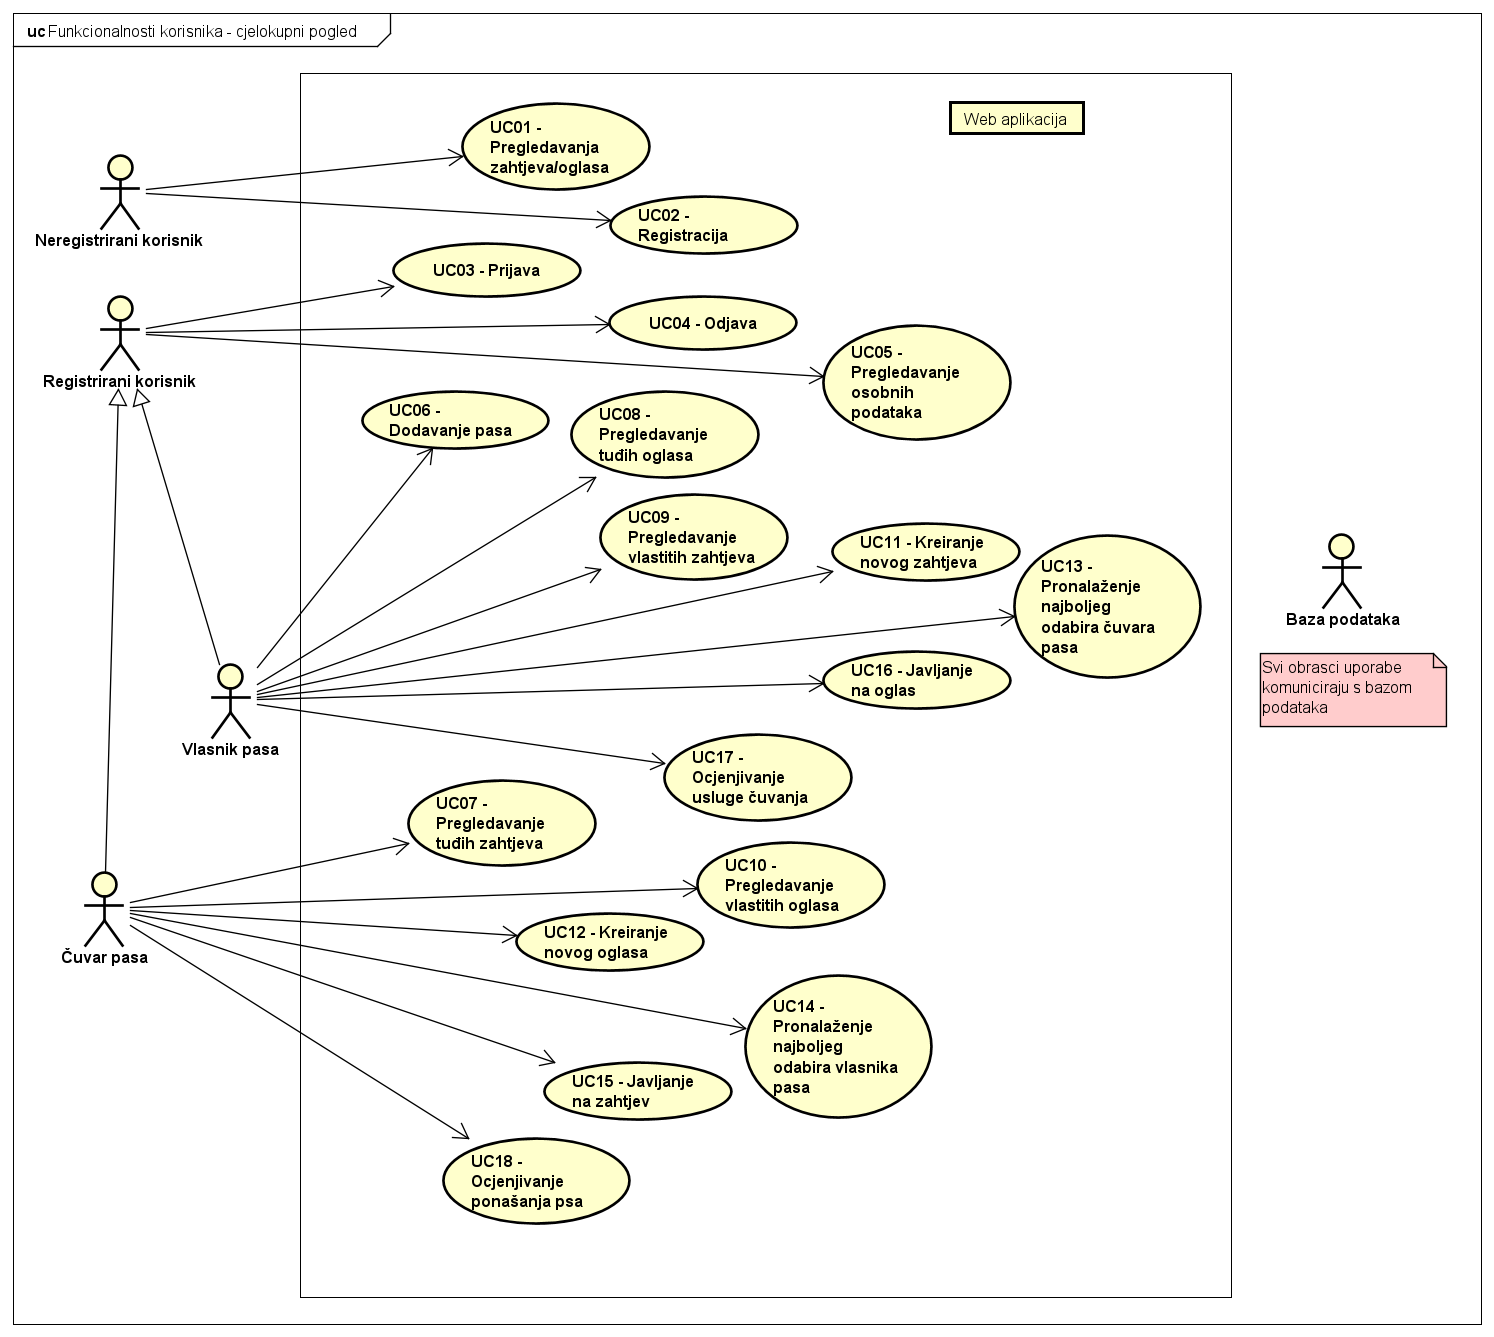
\includegraphics[width=14cm]{slike/Dijagram obrazaca uporabe - korisnik}
						\caption{Dijagram obrasca uporabe - Funkcionalnost neregistriranog korisnika i registriranog korisnika (vlasnika pasa i čuvara pasa)}
						\label{fig:DOU-korisnici}
					\end{figure}
				\eject		
					\begin{figure}[htb]
						\centering
						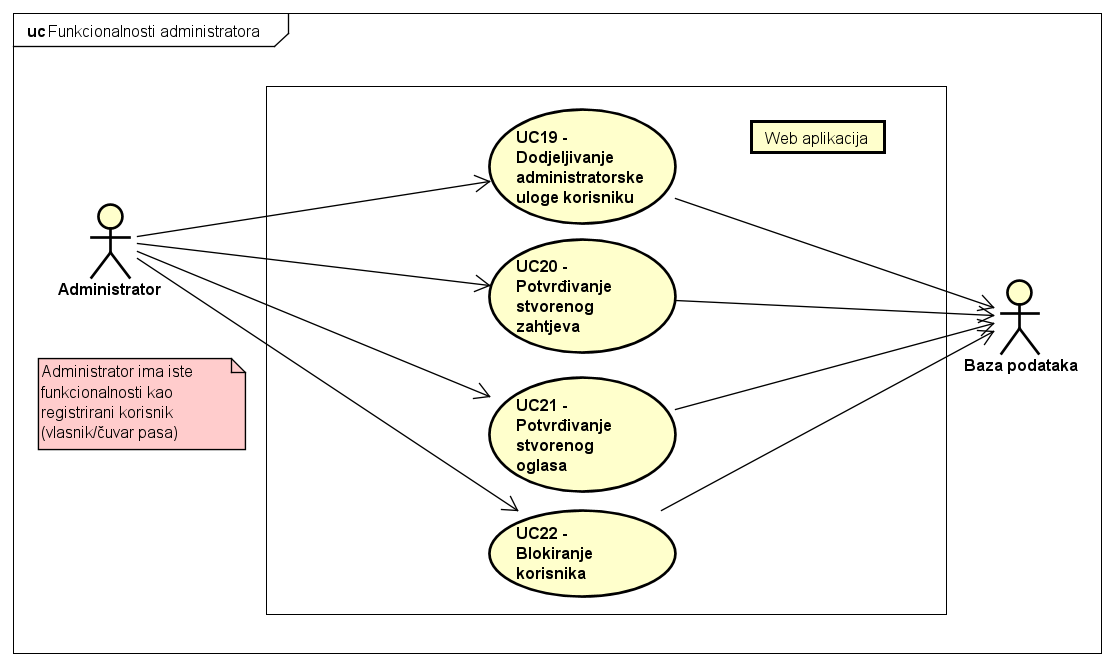
\includegraphics[width=14cm]{slike/Dijagram obrazaca uporabe - administrator}
						\caption{Dijagram obrasca uporabe - Funkcionalnost administratora}
						\label{fig:DOU-administrator}
					\end{figure}
				\eject		
				
			\subsection{Sekvencijski dijagrami}
				
				\textbf{Obrazac uporabe UC11 - Kreiranje novog zahtjeva}\\
				
				Vlasnik pasa na stranici s prikazom vlastitih zahtjeva odabire opciju za kreiranje novog zahtjeva. Web aplikacija mu otvara stranicu za kreiranje zahtjeva. Korisnik tamo unosi tražene podatke (period čuvanja, potrebne aktivnosti itd.) za kreiranje zahtjeva. Potom korisnik potvrđuje kreiranje zahtjeva. Ako korisnik nije ispravno unio podatke, prilikom potvrde web aplikacija ga ponovno usmjerava na istu stranicu s prikladnom porukom o greški. Ako su svi podaci uneseni ispravno, web aplikacija mu daje odgovor o uspješnom kreiranju zahtjeva. Potom se zahtjev pohranjuje u bazu podataka.
				
				\begin{figure}[htb]
					\centering
					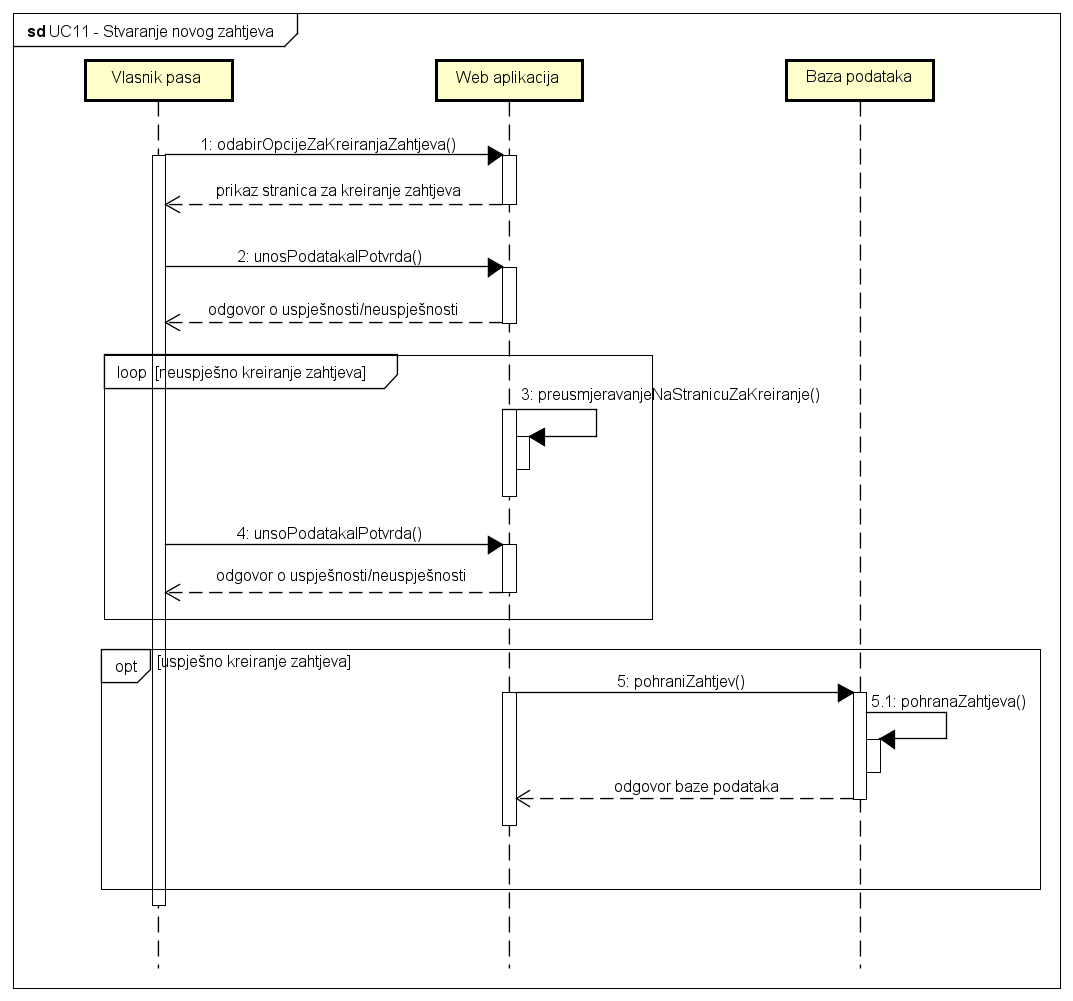
\includegraphics[width=13cm]{slike/Sekvencijski dijagram - UC11}
					\caption{Sekvencijski dijagram za UC11}
					\label{fig:Sekvencijski-UC11}
				\end{figure}
				\eject		
				
				\textbf{Obrazac uporabe UC14 - Pronalaženje najboljeg odabira vlasnika pasa}\\
				
				Čuvar pasa u zaglavlju aplikacije putem padajućeg izbornika odabire opciju za prikaz vlastitih oglasa. Web aplikacija mu otvara stranicu s njegovim oglasima. Korisnik tamo pokraj željenog oglasa odabire opciju za pronalaženje najboljeg odabira. Web aplikacija pronalazi najboljeg vlasnika pasa i šalje ga korisniku. Korisnik ima mogućnost prihvatiti ga, ali i odbiti. Ako korisnik odbije, nema daljnje suradnje s vlasnikom pasa. Ako ga korisnik prihvati, oglas nad kojim je zatražen najbolji odabir se šalje vlasniku pasa. Tada vlasnik pasa ima također opciju prihvatiti suradnju kao i odbiti ju.
				
				\begin{figure}[htb]
					\centering
					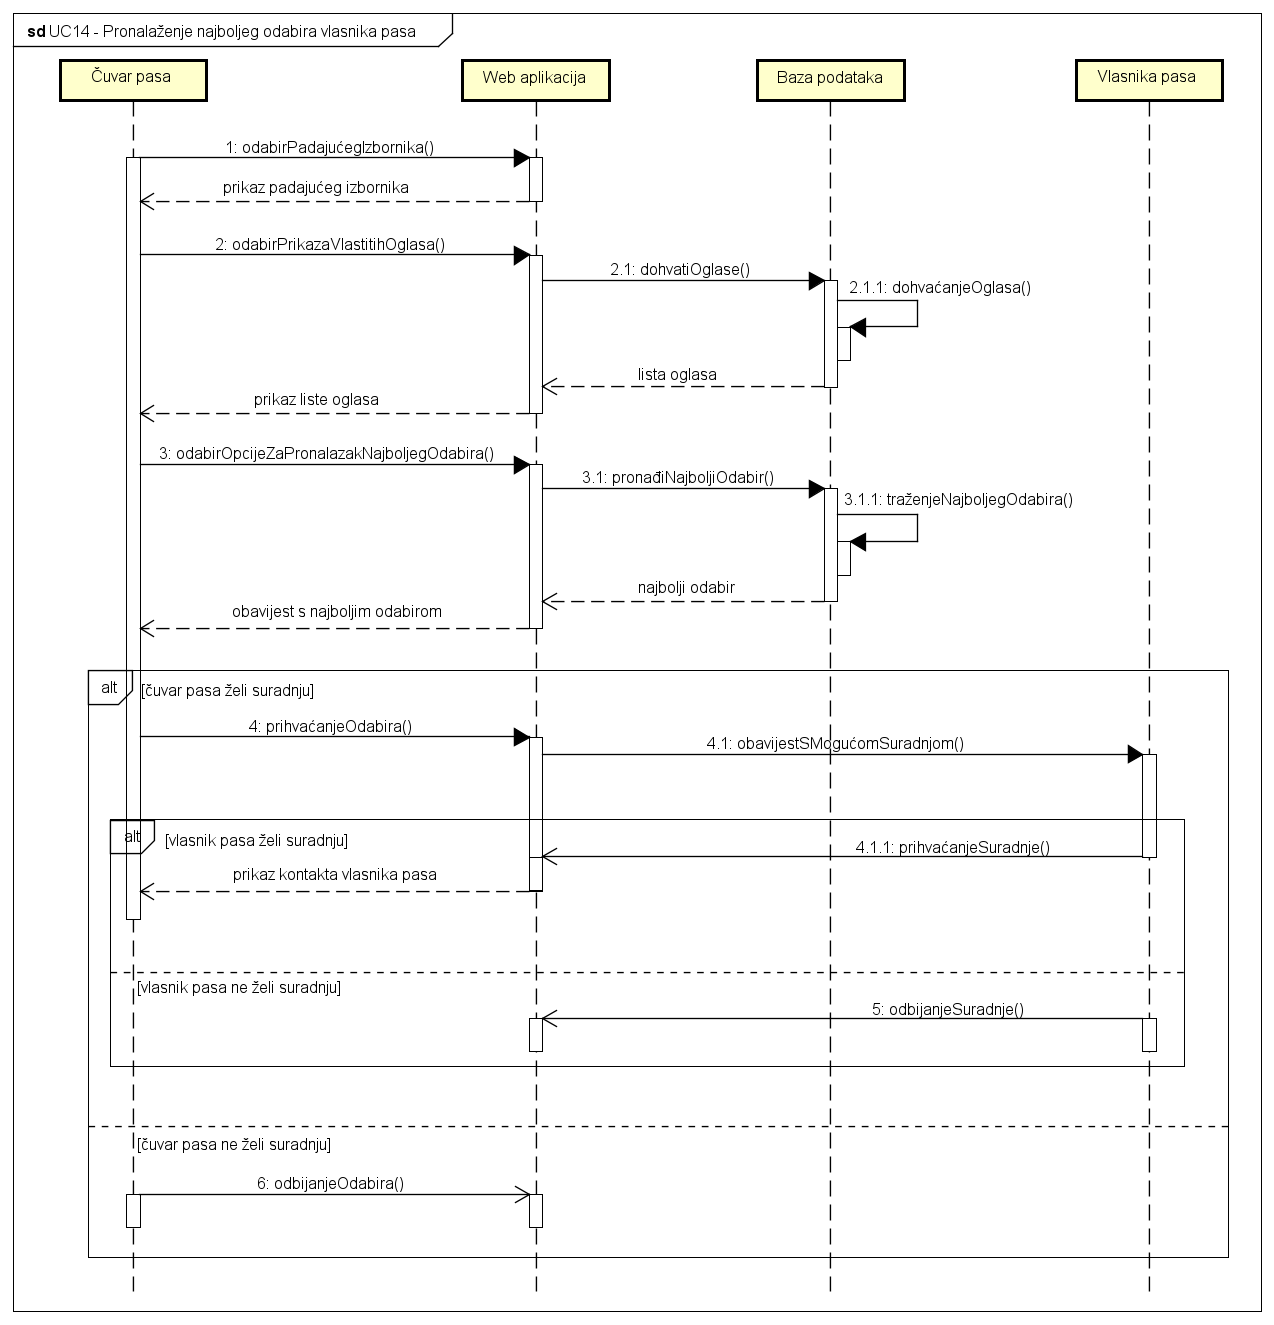
\includegraphics[width=14cm]{slike/Sekvencijski dijagram - UC14}
					\caption{Sekvencijski dijagram za UC14}
					\label{fig:Sekvencijski-UC14}
				\end{figure}
				\eject		
				
				\textbf{Obrazac uporabe UC21 - Potvrđivanje stvorenog zahtjeva}\\
				
				Administrator sustava na početnoj stranici putem padajućeg izbornika odabire opciju za pristupanje stranici za administratorsko upravljanje zahtjevima i oglasima. Web aplikacija šalje upit za potrebnim elementima (svi nepotvrđeni zahtjevi i oglasi) bazi podataka. Primitkom istih, web aplikacija otvara stranicu administratoru. Administrator u listi zahtjeva pronalazi željeni zahtjev te kraj njega odabire opciju za njegovo potvrđivanje. Web aplikacija šalje upit za ažuriranjem zahtjeva bazi podataka. Baza podataka ga ažurira i šalje ažuriranu listu zahtjeva web aplikaciji. Web aplikacija otvara ponovno stranicu administratoru, ali sada s ažuriranom listom zahtjeva i oglasa.
				
				\begin{figure}[htb]
					\centering
					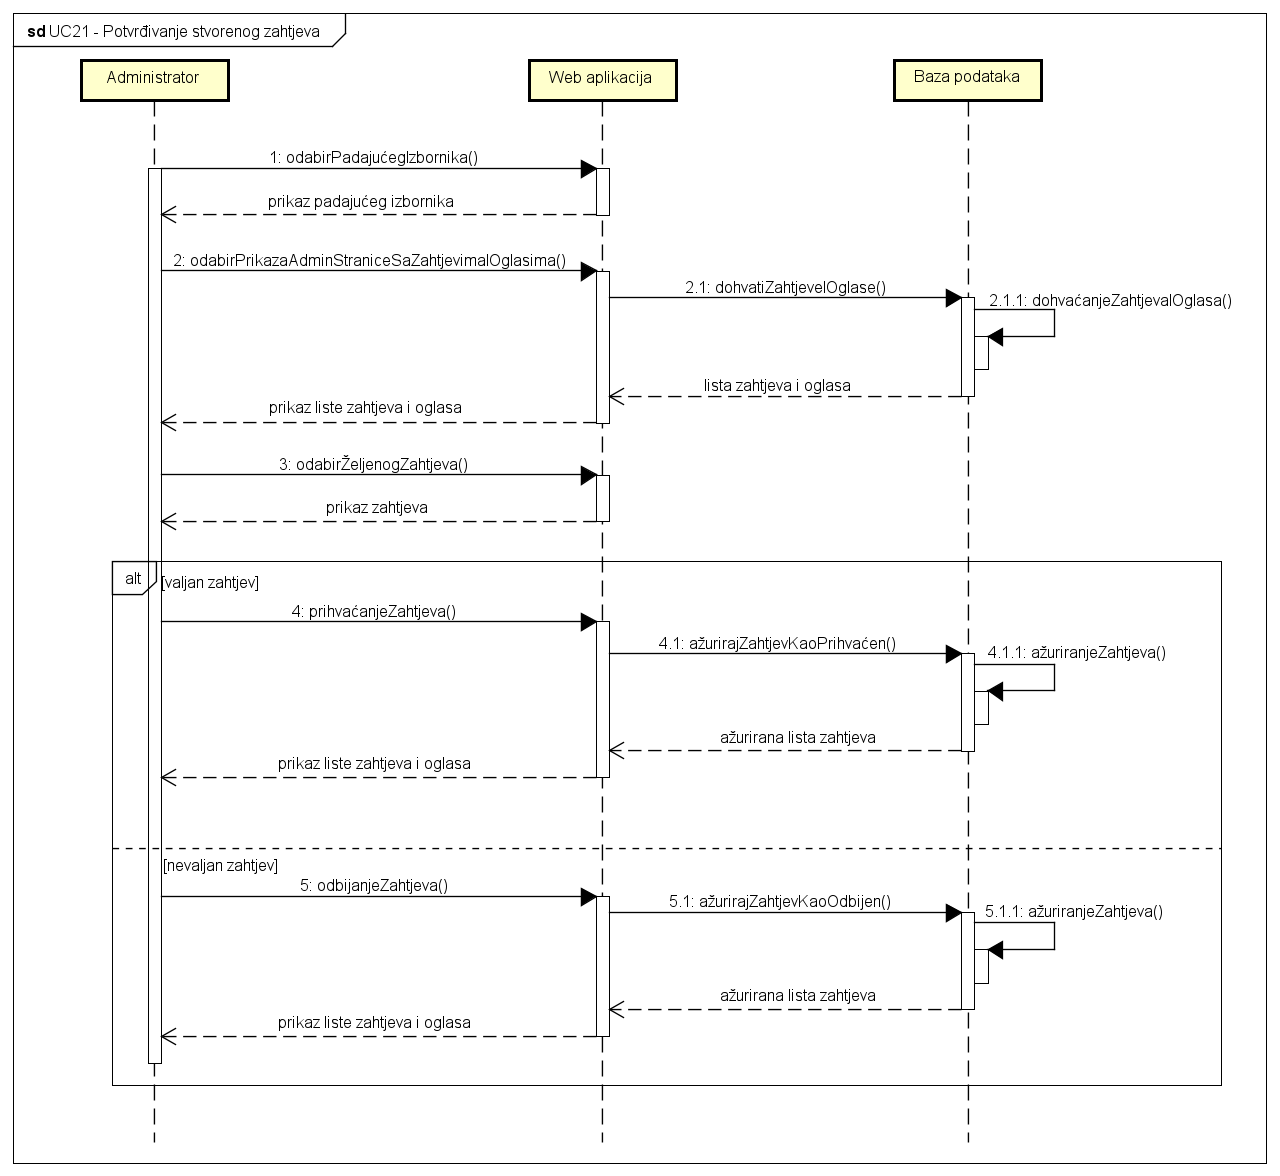
\includegraphics[width=14cm]{slike/Sekvencijski dijagram - UC21}
					\caption{Sekvencijski dijagram za UC21}
					\label{fig:Sekvencijski-UC21}
				\end{figure}
				\eject	
				
				\textbf{Obrazac uporabe UC23 - Blokiranje korisnika}\\
				
				Administrator sustava na početnoj stranici putem padajućeg izbornika odabire opciju za pristupanje stranici za administratorsko upravljanje korisnicima. Web aplikacija šalje upit za potrebnim elementima (svi korisnici sustava) bazi podataka. Primitkom istih, web aplikacija otvara stranicu administratoru. Administrator u listi korisnika pronalazi željenog korisnika te kraj njega odabire opciju za njegovo blokiranje. Web aplikacija šalje upit za ažuriranjem korisnika bazi podataka. Baza podataka postavlja atribut kojim se označava da je korisnik blokiran na istinit i šalje ažuriranu listu korisnika web aplikaciji.
				Web aplikacija otvara ponovno stranicu administratoru, ali sada blokirani korisnik kraj sebe nema gumb za blokiranje.
				
				\begin{figure}[htb]
					\centering
					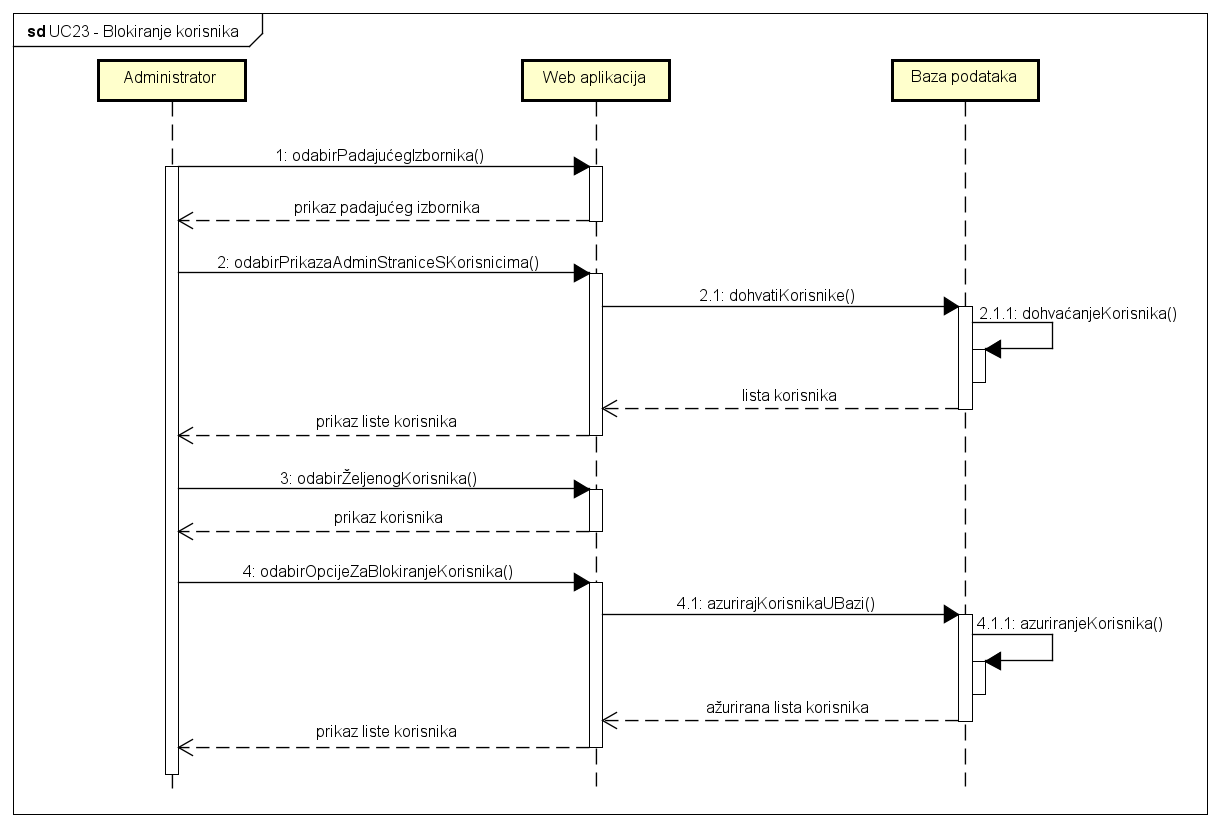
\includegraphics[width=14cm]{slike/Sekvencijski dijagram - UC23}
					\caption{Sekvencijski dijagram za UC23}
					\label{fig:Sekvencijski-UC23}
				\end{figure}
				\eject	
	
		\section{Ostali zahtjevi}
		
			\begin{packed_item}
				
				\item Aplikacija treba biti izvedena kao web aplikacija prilagođena mobilnom uređaju i tabletu
				\item Aplikaciji pristupaju registrirani korisnici uz pomoć korisničkog imena i lozinke
				\item Sustav treba podržavati rad više korisnika u stvarnom vremenu
				\item Aplikaciju treba implementirati u arhitekturi klijent-poslužitelj
				\item Na poslužiteljskoj strani se treba koristit programski jezik Java i radni okvir Spring Boot
				\item Podaci se trebaju spremati u relacijsku bazu podataka koristeći JPA
				\item Funkcionalnost web aplikacije se treba izložiti kroz REST Web servis
				\item Na klijentkoj strani treba implementirati korisničko sučelje u Web pregledniku koristeći React, koje se spaja na navedene servise
			\end{packed_item}
			 
			 
			 
	